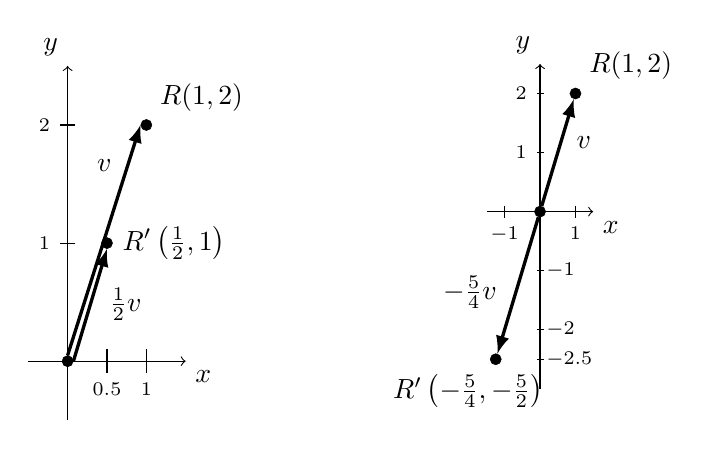
\begin{tikzpicture}[
	point/.style={circle,draw,very thin,fill,inner sep=0pt,minimum size=4pt},
	vector/.style={-latex},
]

	% (1/2)x
	\begin{scope}[yscale=1.5]
		\draw[->] (-0.5,0) to (1.5,0) node[below right] {$x$};
	  \draw[->] (0,-0.5) to (0,2.5) node[above left] {$y$};
		\foreach \x in {0.5,1} {
			\draw (\x,0.1) to (\x,-0.1) node[below] {$\scriptstyle \x$};
		}
		\foreach \y in {1,2} {
			\draw (0.1,\y) to (-0.1,\y) node[left] {$\scriptstyle \y$};
		}
		\node[point] at (0,0) (o) {};
		\node[point] at (1,2) (r) [label=above right:{$R(1,2)$}] {};
		\node[point] at (0.5,1) (r2) [label=right:{$R'\left(\frac{1}{2},1\right)$}] {};
		\draw[vector,very thick] (o.north) to node[above left,near end] {$\uvec{v}$} (r.west);
		\draw[vector,very thick] (o.east) to node[below right,near end] {$\frac{1}{2}\uvec{v}$} (r2.south);
	\end{scope}

	% (-5/4)x
	\begin{scope}[xshift=6cm,yshift=1.9cm,xscale=0.45,yscale=0.75]
		\draw[->] (-1.5,0) to (1.5,0) node[below right] {$x$};
	  \draw[->] (0,-3) to (0,2.5) node[above left] {$y$};
		\foreach \x in {-1,1} {
			\draw (\x,0.1) to (\x,-0.1) node[below] {$\scriptstyle \x$};
		}
		\foreach \y in {1,2} {
			\draw (0.1,\y) to (-0.1,\y) node[left] {$\scriptstyle \y$};
		}
		\foreach \y in {-2.5,-2,-1} {
			\draw (0.1,\y) to (-0.1,\y) node[right] {$\scriptstyle \y$};
		}
		\node[point] at (0,0) (o) {};
		\node[point] at (1,2) (r) [label=above right:{$R(1,2)$}] {};
		\node[point] at (-1.25,-2.5) (r2) [label=below:{$R'\left(-\frac{5}{4},-\frac{5}{2}\right)\qquad$}] {};
		\draw[vector,very thick] (o) to node[below right,near end] {$\uvec{v}$} (r);
		\draw[vector,very thick] (o) to node[above left,near end] {$-\frac{5}{4}\uvec{v}$} (r2);
	\end{scope}

\end{tikzpicture}
